\documentclass[10pt]{article}
\usepackage[utf8]{inputenc}
\usepackage[T1]{fontenc}
\usepackage{graphicx}
\usepackage[export]{adjustbox}
\graphicspath{ {./images/} }
\usepackage{amsmath}
\usepackage{amsfonts}
\usepackage{amssymb}
\usepackage[version=4]{mhchem}
\usepackage{stmaryrd}

\title{Air Gap }

\author{}
\date{}


\begin{document}
\maketitle
\includegraphics[max width=\textwidth]{Airgap}

A physical separation between the free-flowing discharge end of a potable water supply pipeline and an open or non-pressure receiving vessel. Should not be used in an area with dangerous atmosphere.

An "approved air gap" shall be at least twice the diameter of the supply pipe measured vertically above the overflow rim of the receiving vessel; in no case less than 1 inch $(2.54 \mathrm{~cm})$.

\textbf{Common Applications - Lethal hazards (raw sewage, recycled water, auxiliary water supply}

\section{Atmospheric Vacuum Breaker Assembly (AVB)}
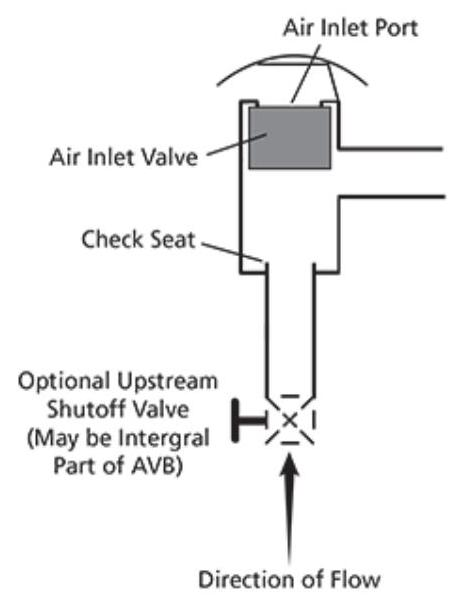
\includegraphics[max width=\textwidth]{AtmosphericVacuumBreaker(2)}

An assembly containing an air inlet valve, a check seat and an air inlet port(s). (Also known as the non-pressure type vacuum breaker.) The flow of water into the body causes the air inlet valve to close the air inlet port(s). When the flow of water stops the air inlet valve falls and forms a check valve against backsiphonage. At the same time it opens the air inlet port(s) allowing air to enter and satisfy the vacuum. A shutoff valve immediately upstream may be an integral part of the assembly, but there shall be no shutoff valves or obstructions downstream. The assembly shall not be subjected to operating pressure for more than twelve (12) hours in any twenty-four (24) hour period.

An atmospheric vacuum breaker is designed to protect against a non-health hazard (i.e., pollutant) or a health hazard (i.e., contaminant) under a backsiphonage condition only.

Common Applications - Irrigation systems
\newpage
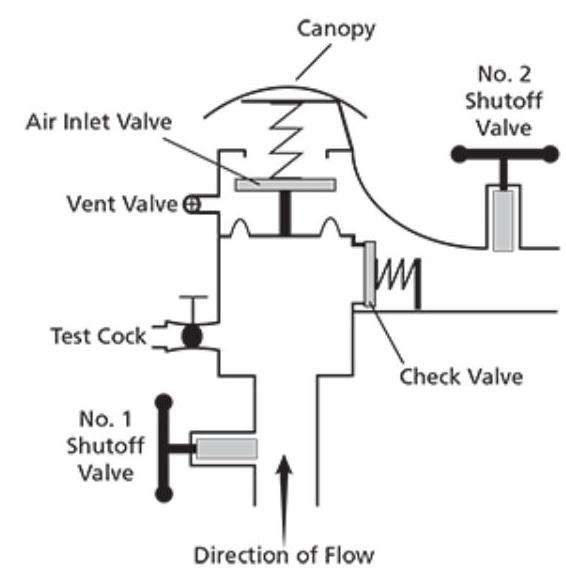
\includegraphics[max width=\textwidth]{PressureVacuumBreaker(2)}

Direction of Flow An assembly containing an independently operating internally loaded check valve and an independently operating loaded air inlet valve located on the discharge side of the check valve. The assembly is to be equipped with properly located resilient seated test cocks and tightly closing resilient seated shutoff valves attached at each end of the assembly.

This assembly is designed to protect against a non-health hazard(i.e., pollutant) or a health hazard (i.e., contaminant) under a backsiphonage condition only.

Common Applications - Irrigation systems
\newpage
\section{Spill-Resistant Vacuum Breaker Assembly (SVB)}
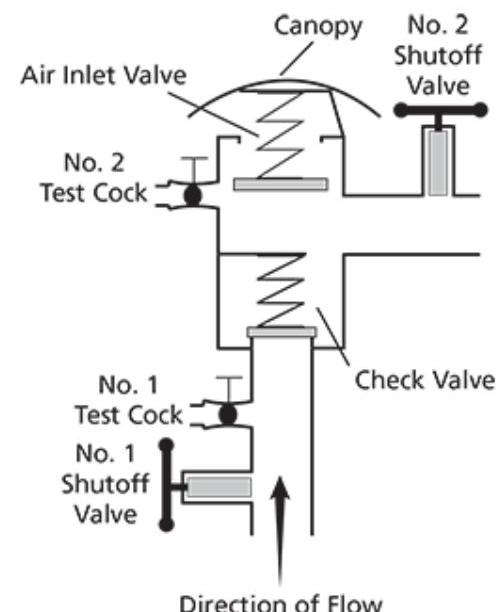
\includegraphics[max width=\textwidth]{SpillResitantVacuumBreaker}

An assembly containing an independently operating internally loaded check valve and independently operating loaded air inlet valve located on the discharge side of the check valve. The assembly is to be equipped with a properly located resilient seated test cock, a properly located bleed/vent port, and tightly closing resilient seated shutoff valves attached at each end of the assembly.

This assembly is designed to protect against a non-health hazard(i.e., pollutant) or a health hazard (i.e., contaminant) under a backsiphonage condition only.

Common Applications - Irrigation systems
\newpage
\section{Double Check Valve Assembly}
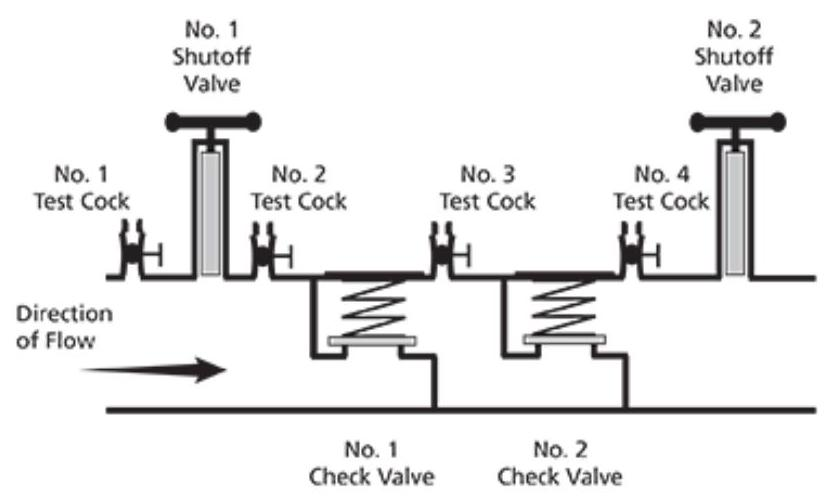
\includegraphics[max width=\textwidth]{DoubleCheckValve}

An assembly composed of two independently acting, approved check valves, including tightly closing resilient seated shutoff valves attached at each end of the assembly and fitted with properly located resilient seated test cocks.

This assembly shall only be used to protect against a non-health hazard (i.e., pollutant)

\textbf{Common Applications: } - Fire sprinkler systems, non-hazardous irrigation, combi-boilers, non-health hazards
\newpage
\section{Double Check Detector Assembly (DCDA)}
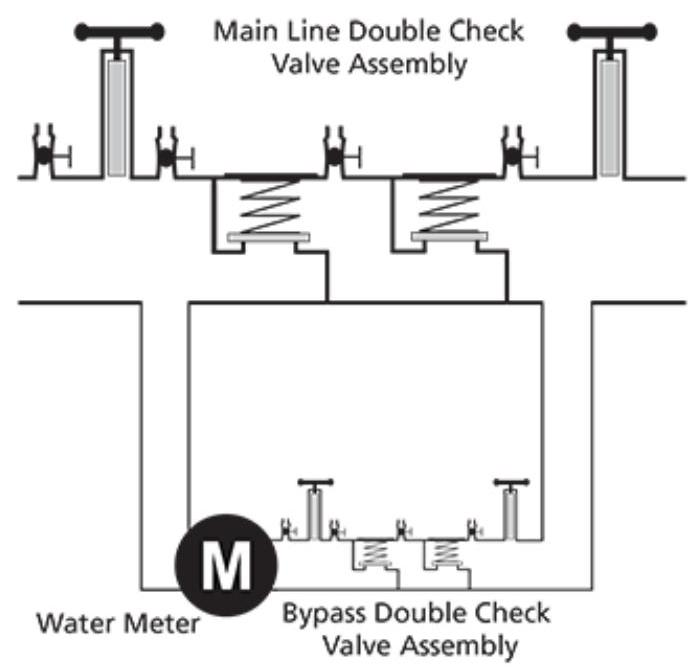
\includegraphics[max width=\textwidth]{DoubleCheckDetector}

A specially designed assembly composed of a linesize approved double check valve assembly with a bypass containing a specific water meter and an approved double check valve assembly. The meter shall register accurately for rates of flow up to $2 \mathrm{gpm}$ (gallons per minute) and shall show a registration for all rates of flow.

This assembly shall only be used to protect against a non-health hazard (i.e., pollutant). The DCDA is primarily used on fire sprinkler systems

\textbf{Common Applications: } - Fire sprinkler systems (detects low flow on static line)
\newpage
\section{Reduce Pressure Principle Assembly}
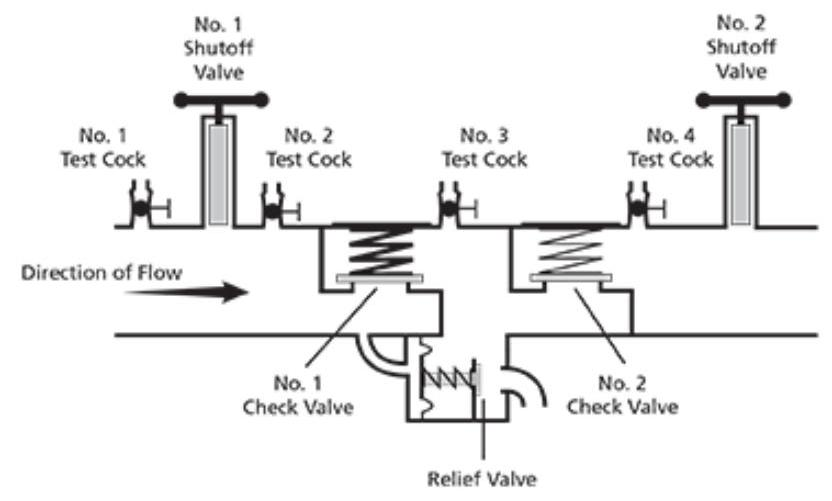
\includegraphics[max width=\textwidth]{ReducedPressurePrinciple}

An assembly containing two independently acting approved check valves together with a hydraulically operating, mechanically independent pressure differential relief valve located between the check valves and at the same time below the first check valve. The unit shall include properly located resilient seated test cocks and tightly closing resilient seated shutoff valves at each end of the assembly.

This assembly is designed to protect against a non-health hazard(i.e., pollutant) or a health hazard (i.e., contaminant).

This assembly shall not be used for backflow protection of sewage or reclaimed water. (Note: Check with local administrative authority for acceptable uses.

\textbf{Common Applications: } - Domestic water and irrigation service protection, health hazards
\newpage
\section{Reduced Pressure Principle Detector Assembly}
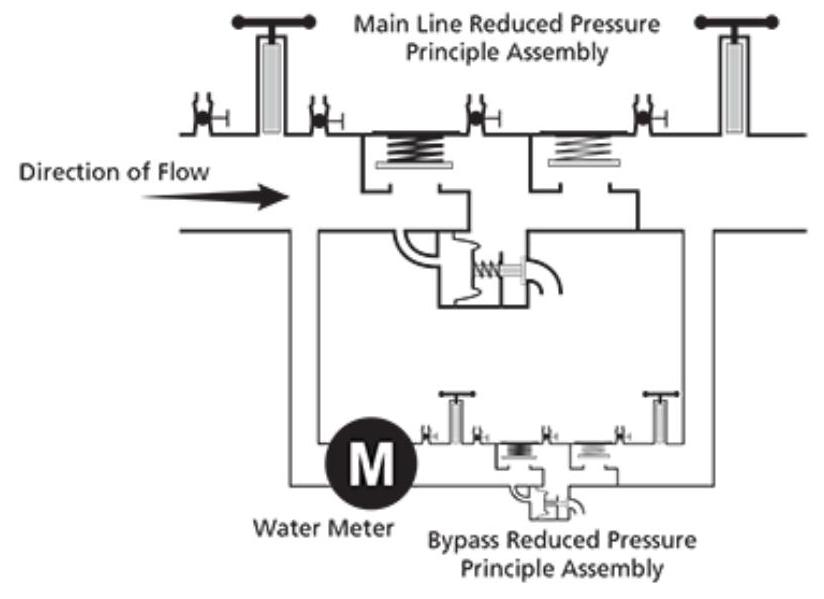
\includegraphics[max width=\textwidth]{ReducedPressurePrincipleDetector}

A specially designed assembly composed of a linesize approved reduced pressure principle backflow prevention assembly with a specific bypass containing a specific water meter and an approved reduced pressure principle backflow prevention assembly. The meter shall register accurately for rates of flow up to $2 \mathrm{gpm}$ and shall show a registration for all rates of flow. (See Chapter 10, for additional details.)

This assembly shall be used to protect against a non-health hazard (i.e., pollutant) or a health hazard (i.e., contaminant). The RPDA is primarily used on fire sprinkler systems.

\textbf{Common Applications: } - Fire sprinkler systems (detects low flow on static line)


\end{document}